\item A thin conducting rod MN of mass 20 g, length 25 cm and resistance 10 $\Omega$ is held on frictionless, long, perfectly conducting vertical rails as shown in the figure. There is a uniform magnetic field $B_0 = 4 \, \text{T}$ directed perpendicular to the plane of the rod-rail arrangement. The rod is released from rest at time $t = 0$ and it moves down along the rails. Assume air drag is negligible. Match each quantity in List-I with an appropriate value from List-II, and choose the correct option.\\[2 mm]

[\textbf{Given:}] The acceleration due to gravity $g = 10 \, \text{m s}^{-2}$ and $e^{-1} = 0.4$ 

\begin{center}
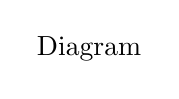
\begin{tikzpicture}
\node {Diagram};
\end{tikzpicture}
\end{center}



\begin{center}
\renewcommand{\arraystretch}{2}
\begin{table}[h]
    \centering
    \begin{tabular}{p{0.25cm}p{9cm}|p{0.25cm}p{4cm}}
    \hline
    & Column I & & Column II \\
    \hline
    (A) & At $t = 0.2 \, \text{s}$, the magnitude of the induced emf in Volt & (1) & 0.07 \\
    (B) & At $t = 0.2 \, \text{s}$, the magnitude of the magnetic force in Newton & (2) & 0.14 \\
    (C) & At $t = 0.2 \, \text{s}$, the power dissipated as heat in Watt & (3) & 1.20 \\
    (D) & The magnitude of terminal velocity of the rod in $\text{m s}^{-1}$ & (4) & 0.12 \\
     &  & (5) & 2.00 \\
    \hline
    \end{tabular}
\end{table}
\end{center}

\begin{tasks}(2)
    \task $P \rightarrow 5, (Q) \rightarrow 2, (R) \rightarrow 3, (S) \rightarrow 1$
    \task $P \rightarrow 3, (Q) \rightarrow 1, (R) \rightarrow 4, (S) \rightarrow 5$
    \task $P \rightarrow 4, (Q) \rightarrow 3, (R) \rightarrow 1, (S) \rightarrow 2$
    \task $P \rightarrow 3, (Q) \rightarrow 4, (R) \rightarrow 2, (S) \rightarrow 5$\ans
\end{tasks}